\chapter{\IfLanguageName{dutch}{Stand van zaken}{State of the art}}%
\label{ch:stand-van-zaken}
% Tip: Begin elk hoofdstuk met een paragraaf inleiding die beschrijft hoe
% dit hoofdstuk past binnen het geheel van de bachelorproef. Geef in het
% bijzonder aan wat de link is met het vorige en volgende hoofdstuk.

% Pas na deze inleidende paragraaf komt de eerste sectiehoofding.

%%Dit hoofdstuk bevat je literatuurstudie. De inhoud gaat verder op de inleiding, maar zal het onderwerp van de bachelorproef *diepgaand* uitspitten. De bedoeling is dat de lezer na lezing van dit hoofdstuk helemaal op de hoogte is van de huidige stand van zaken (state-of-the-art) in het onderzoeksdomein. Iemand die niet vertrouwd is met het onderwerp, weet nu voldoende om de rest van het verhaal te kunnen volgen, zonder dat die er nog %%andere informatie moet over opzoeken \autocite{Pollefliet2011}.

%%Je verwijst bij elke bewering die je doet, vakterm die je introduceert, enz.\ naar je bronnen. In \LaTeX{} kan dat met het commando \texttt{$\backslash${textcite\{\}}} of \texttt{$\backslash${autocite\{\}}}. Als argument van het commando geef je de ``sleutel'' van een ``record'' in een bibliografische databank in het Bib\LaTeX{}-formaat (een tekstbestand). Als je expliciet naar de auteur verwijst in de zin (narratieve referentie), gebruik je \texttt{$\backslash${}textcite\{\}}. Soms is de auteursnaam niet expliciet een onderdeel van de zin, dan gebruik je \texttt{$\backslash${}autocite\{\}} (referentie tussen haakjes). Dit gebruik je bv.~bij een citaat, of om in het bijschrift van een overgenomen afbeelding, broncode, tabel, enz. te %%verwijzen naar de bron. In de volgende paragraaf een voorbeeld van elk.

%%\textcite{Knuth1998} schreef een van de standaardwerken over sorteer- en zoekalgoritmen. Experten zijn het %%erover eens dat cloud computing een interessante opportuniteit vormen, zowel voor gebruikers als voor %%dienstverleners op vlak van informatietechnologie~\autocite{Creeger2009}.

%%Let er ook op: het \texttt{cite}-commando voor de punt, dus binnen de zin. Je verwijst meteen naar een bron in %%de eerste zin die erop gebaseerd is, dus niet pas op het einde van een paragraaf.
%%\lipsum[7-20]
\section{Navigatie}
\label{sec:navigatie}
Navigatie is de kunst van het plannen en volgen van een route om zich daarmee van de huidige positie naar de bestemming te verplaatsen. Het woord 'navigatie' is afgeleid uit de Latijnse woorden navis, dat schip betekent, en agere, dat in deze context bewegen of sturen betekent. Bij navigatie gaat het erom dat je je eigen plaats bepaald en de plaats bepaald waar je heen gaat en daarna de weg er naar toe. \textcite{Katz2010} introduceerde het NAVIG-systeem, dat GNSS (Global Navigation Satellite System) en snelle visuele herkenning combineert om visueel gehandicapte gebruikers te begeleiden in zowel bekende als onbekende omgevingen. Deze systemen benadrukken het belang van technologie voor het verbeteren van navigatie voor mensen met een beperking. Om hier iets aan te doen, ontwikkelde \textcite{Lakde2015} een navigatiehulpsysteem voor visueel gehandicapten, dat gebruik maakt van een combinatie van sensortechnologie en stembegeleiding. Dit systeem maakt gebruikers bewust van hun pad en eventuele obstakels. Navigatie, zoals gedefinieerd door \textcite{Gachet2010}, is de handeling van het bewegen door een onbekende omgeving, en kan met name een uitdaging zijn voor visueel gehandicapten.
\section{Mentale Beperking}
\label{sec:mentale beperking}
Het begrip "verstandelijke handicap" of mentale beperking wordt door het Vlaams Agentschap voor Personen met een Handicap (VAPH) gedefinieerd aan de hand van richtlijnen van de DSM-5, de American Association on Intellectual and Developmental Disabilities (AAIDD), en het Classificerend Diagnostisch Protocol (CDP). Volgens de American Psychiatric Association (APA) betreft een verstandelijke handicap een stoornis die ontstaat tijdens de ontwikkeling en zowel beperkingen in intellectueel functioneren als aanpassingsproblemen op conceptueel, sociaal en praktisch niveau omvat. De benadering van het VAPH richt zich op het sociaal-ecologische perspectief, waarbij het functioneren van individuen wordt gezien als een interactie tussen de persoon en zijn omgeving. Het verkrijgen van ondersteuning bij dagelijkse activiteiten staat hierbij centraal, waarbij zowel persoonlijke als externe factoren van invloed zijn op het functioneren. Het is van belang dat bij het vaststellen van een verstandelijke handicap ook rekening wordt gehouden met de sterke punten van de betrokkene. Om de diagnose van een verstandelijke handicap te stellen, moeten drie criteria worden voldaan: het intelligentiecriterium, het criterium adaptief gedrag en het ontwikkelingscriterium. Het intelligentie criterium vereist een aantoonbare beperking in intellectueel functioneren, vaak vastgesteld met gestandaardiseerde intelligentietests. Het criterium adaptief gedrag omvat tekorten in aanpassingsgedrag op conceptueel, sociaal en praktisch gebied. Het ontwikkelingscriterium vereist dat deze beperkingen zich manifesteren vóór de leeftijd van 22 jaar. Personen met een verstandelijke handicap kunnen verder worden onderverdeeld op basis van de ernst ervan, wat voornamelijk voor onderzoeks- en rapportagedoeleinden wordt gedaan. Het gebruik van deze onderverdeling in de praktijk vereist echter zorgvuldige afweging, zoals beschreven in het diagnostisch protocol \autocite{VAPH}.
\section{Augmented Reality}
\label{sec:augmented reality}
Augmented Reality (AR) is een technologie die de gebruikerservaring verbetert door digitale informatie over objecten of plaatsen in de echte wereld te projecteren (Berryman, 2012). Het verschilt van virtual reality (VR) doordat gebruikers nog steeds hun fysieke omgeving ervaren \autocite{Calo2015}. AR wordt op verschillende gebieden gebruikt, waaronder geneeskunde, marketing en onderwijs, en wordt gedefinieerd als een realtime weergave van de fysieke wereld, versterkt door virtueel computergegenereerde informatie \autocite{Carmigniani2011}. Het is een veelzijdige technologie met potentiële positieve toepassingen, maar brengt ook beleidszorgen met zich mee die moeten worden aangepakt \autocite{Calo2015}. Er zijn verschillende soorten beleidsvormen. Het bouwen van dynamische systemen die flexibel zijn en kunnen bijgewerkt worden naarmate de technologie en cultuur veranderen. AR wordt anders ervaren voor verschillende mensen dus het is belangrijk diverse bevolkingsgroepen te raadplegen. De data bescherming is belangrijk naar wat kan en niet zodat het systeem ook geen vooroordelen trekt op vlak van bepaalde verkeerde gevoede data. De algemene conclusie hieruit is dat AR-systemen ontwikkelt moeten worden zodanig dat deze gemakkelijk aanpasbaar naarmate de verandering in technologie en samenleving \autocite{Calo2015}.
\section{Artificiële Intelligentie}
\label{sec:artificiële intelligentie}
Artificiële Intelligentie (AI) is het vermogen van een machine of computersysteem om taken te simuleren en uit te voeren die menselijke intelligentie vereisen, zoals logisch redeneren, leren en problemen oplossen. AI is gebaseerd op het gebruik van algoritmen en technologieën voor machinaal leren om machines in staat te stellen bepaalde cognitieve vaardigheden na te bootsen. Naarmate AI zich verder ontwikkelt, kan het naar verwachting de efficiëntie van veel processen verbeteren en mensen helpen om complexe taken sneller en nauwkeuriger uit te voeren \autocite{Sabouret2020}. AI kan het mogelijk maken in ons gebied van onderzoek de relatief beste route te bereken en tevens de beste manier om eenvoudig op de bestemming te geraken \autocite{Soni2023a}. Het gebruik van datastructuren zal toelaten deze locatie informatie te linken aan het routepatroon \autocite{Ruta2010}. Deze patronen kunnen potentiële knelpunten identificeren, hulp bieden bij het optimaliseren van routes als er verkeerswerken of files zijn. De noodzaak van dit systeem zijn realtime gegevens \autocite{Ciravegna2018}.
\section{Hedendaagsevormen of factors van navigatie}
\label{sec:literatuuroverzicht}
\subsection{Google maps}
\label{sec:google maps}
Google maps\footnote{\url{https://www.google.com/maps}} is een gebruikersvriendelijke ervaring voor gewone gebruikers om locaties te zoeken, routes te plannen en navigatie-instructies te ontvangen. Een standaardprocedure voor een normaal persoon zou zijn:
\begin{enumerate}
    \item De gebruiker geeft een de naam van de bestemming in.
    \item Hierna kan de gebruiker kiezen voor route waarbij Google maps automatisch de beste mogelijke routes teruggeeft.
    \item Als laatste geeft de applicatie onderweg stapsgewijze instructies met auditieve geluiden of visuele kaartbegeleiding.
\end{enumerate}
Voor mensen met een mentale beperking kan hier de blokkade zijn de cognitieve overbelasting. De complexiteit van de interface en de hoeveelheid informatie die ze terug krijgen kan mogelijke hinder vormen in het begrijpen en verwerken van deze informatie. Navigatieverwarring kan een ander mogelijks probleem hierbij vormen, bepaalde instructies zijn te complex gevormd of onduidelijk. Deze applicatie heeft vele voordelen zoals real-time verkeersinformatie. Google Maps maakt gebruikt van real-time gegevens en hiermee kunnen ze bepaalde verkeersomstandigheden of vertragingen vermijden. De functie Street View die Google Maps aanbied kan hele goede visuele beelden opleveren voor mensen met een beperking zodat ze het gevoel krijgen dat ze daar fysiek aanwezig zijn. Dit kan heel handig zijn bij het vooraf plannen van routes. Het grootste probleem met deze applicatie is de privacy. Het gebruik maken van real-time gegevens komt ten koste van heel wat locatie data. Een internetverbinding is vereist voor het gebruiken van deze applicatie. Als laatste Google voegde onlangs hun AR technologie: GoogleARVR\footnote{\url{https://arvr.google.com}} toe aan de applicatie Google Maps. Je kan deze gebruiken voor bekende plekken te bezoeken of gaan verkennen van de omgeving in AR.
\begin{figure}
\centering
\captionsetup{justification=centering}
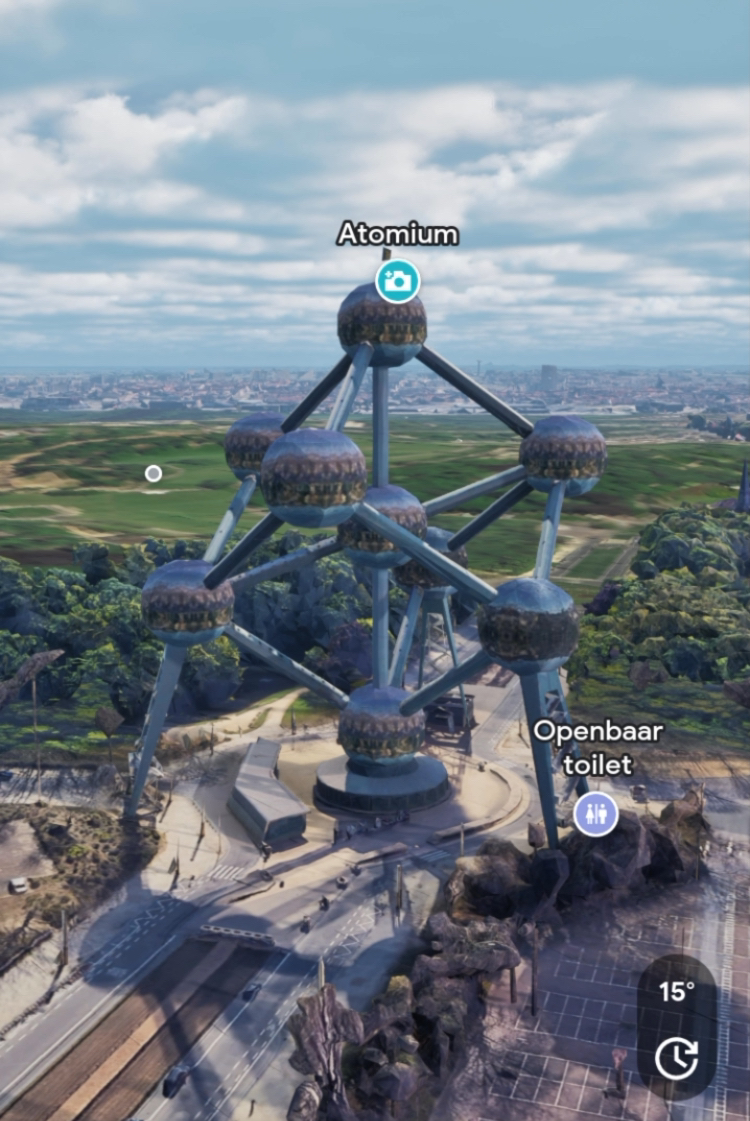
\includegraphics[width=0.5\textwidth]{IMG_1}
\caption[Immersive view Atomium Brussels]{Immersive view Atomium Brussels}
\end{figure}
\subsection{Mapbox}
\label{sec:mapbox}
Mapbox\footnote{\url{https://www.mapbox.com}} biedt een platform voor het maken en integreren van aangepaste kaarten en locatiegebaseerde services. De kaartweergave van Mapbox biedt verschillende kaartstijlen en aanpasbare kaartlagen, waardoor gebruikers een breed scala aan visuele informatie kunnen verkennen. Dit platform is ontworpen voor applicaties van derden, zo kunnen de navigatiediensten geïntegreerd worden in hun applicaties voor routebegeleiding en route-algoritmen. Mapbox heeft als groot voordeel de aanpasbaarheid per gebruiksgeval, zo kan het gemakkelijk aangepast worden naar specifieke behoeften en gebruikerservaringen. Het platform biedt AR/VR toepassingen aan, dit versterkt de leer mogelijkheden voor mensen met mentale beperking. Het grootste nadeel in deze applicatie is de afhankelijkheid van een ontwikkelaar. Ook de complexiteit die uit de applicatie komt kan mogelijke vaardigheden vereisen.
\subsection{Sygic}
\label{sec:sygic}
Sygic\footnote{\url{https://www.sygic.com/nl}} is een navigatie-app die gebruikers helpt bij het plannen van routes, navigeren op de weg en het vermijden van verkeersopstoppingen. De standaardprocedure voor het platform is je geeft je bestemming in en het programma berekent de beste route op basis van actuele verkeersinformatie. Tijdens het verplaatsen ontvangt de gebruikers stapsgewijze instructies aan de hand van spraaknavigatie, meldingen voor afslagen, rotondes en andere manoeuvres. Eens je jouw route hebt ingeladen kan je de verplaatsing offline verder zetten zonder actuele internetverbinding. Sommige geavanceerde functie van Sygic, zoals bepaalde voorkeuren instellen of het vinden van een specifiek punt. Het grootste probleem met Sygic is dat de software gebouwd is voor auto navigatie.
\subsection{De Lijn}
\label{sec:delijn}
De Lijn\footnote{\url{https://www.delijn.be/nl/routeplanner/}} staat in voor alles rond het bus en tram netwerk in Vlaanderen. Hun applicatie werkt als volgt je geeft je vertrek- en aankomstpunt in. De applicatie geeft dan een lijst terug met mogelijke bussen of trams om efficiënt op jouw bestemming te geraken. Bij het ingeven van je vertrek- en aankomstpunt geeft het ingebouwde systeem ook meteen de dichtstbijzijnde halte weer en hoe ver het wandelen is van deze halte tot je bestemming. Het systeem biedt ook real-time gegevens aan over de bussen en trams. De complexiteit van de applicatie kan een cruciale rol spelen in het verplaatsen van zichzelf en de internetverbinding die vereist is.
\subsection{NMBS}
\label{sec:nmbs}
Nationale Maatschappij der Belgische Spoorwegen (NMBS)\footnote{\url{https://www.belgiantrain.be/nl}} is de nationale treindienst van België. De grootste blokkade hier begint al bij het kennen van de vertrek en aankomsthalte. Deze applicatie biedt wel enkele voordelen zoals real-time informatie van de treintijden en het ticket systeem is in staat tickets online te bewaren. Specifieke problemen die zich hier kunnen voordoen is de complexiteit van de interface van de applicatie en een internetverbinding is vereist voor het gebruik van dit platform. In het algemeen loopt deze applicatie zeer analoog met die van De Lijn.
\section{Requirements}
\label{sec:requirements}
Bekijken welke tools voldoen aan de beste requirements 1-2 tools

Vragen aan co-promotor
\section{Het bepalen van de geschikte navigatiemethode}
\label{sec:het bepalen van de geschikte navigatiemethode}
\section{Technologieën}
\label{sec:technologieën}
\subsection{Javascript}
\label{sec:javascript}
JavaScript is een scripttaal waarmee je statische webapplicaties kunt verbeteren met
dynamische, gepersonaliseerde en interactieve inhoud. Dit verbetert de ervaring van bezoekers op uw site en
maakt het waarschijnlijker dat ze opnieuw langskomen. U hebt vast de flikkerende uitklapmenu's, bewegende
tekst en veranderende inhoud die nu wijdverspreid zijn op websites. Ze worden mogelijk gemaakt door JavaScript. JavaScript wordt ondersteund door alle grote browsers en is de taal bij uitstek op het web. Het kan zelfs worden gebruikt buiten webapplicaties, bijvoorbeeld om administratieve taken te automatiseren \autocite{Wilton2004}.
\subsection{React}
\label{sec:react}
React is een bibliotheek waarmee ontwikkelaars gebruikersinterfaces (UI's) kunnen bouwen als een boom van kleine stukjes die componenten worden genoemd. Een component is een mix van HTML en JavaScript die alle logica bevat die nodig is om een klein deel van een grotere UI weer te geven. Elk van deze componenten kan worden opgebouwd tot opeenvolgende complexe onderdelen van een app \autocite{Baer2018}.
\subsection{React Native}
\label{sec:react native}
React Native is een populair open-source framework, dat is ontwikkeld door Facebook. Ontwikkelaars kunnen hiermee mobiele applicaties bouwen aan de hand van JavaScript. React Native applicaties gebruiken de kracht van React, een JavaScript bibliotheek, voor het bouwen van gebruikersinterfaces met mobiele componenten. Door deze componenten kunnen ontwikkelaars efficiënt applicaties maken die werken voor zowel iOS als Android apparaten \autocite{Vinnik2021}.